% !TEX program = pdflatex
\documentclass[3p,11pt]{elsarticle}
\usepackage{amsmath,amssymb}
\usepackage{array}
\usepackage{booktabs}
\usepackage[tableposition=top]{caption}
\usepackage{enumitem}
\usepackage{tikz}
\usepackage{pgfplots}
\pgfplotsset{compat=1.18}
\usepackage{url}
\urlstyle{same}
\usepackage[hidelinks]{hyperref}
\emergencystretch=3em
% first-page footer: the page number alone
\makeatletter
\def\ps@pprintTitle{\let\@oddhead\@empty\let\@evenhead\@empty
  \def\@oddfoot{\hfil\thepage\hfil}\let\@evenfoot\@oddfoot}
\makeatother

% ---- notation ---------------------------------------------------------------
\newcommand{\um}{\,$\mu$m}
\newcommand{\kms}{km\,s$^{-1}$}
\newcommand{\flux}{erg\,cm$^{-2}$\,s$^{-1}$}
\newcommand{\mA}{m\AA}
\newcommand{\sci}[2]{#1\times10^{#2}}
\newcommand{\ion}[2]{#1\,\textsc{#2}}
\newcommand{\nuc}[2]{$^{#1}$#2}
\newcommand{\lxl}{$L_X/L_\mathrm{bol}$}

\begin{document}

\begin{frontmatter}

\title{No hydrogen at the Wow!\ signal's velocity in its two candidate fields}

\author{Charles C. Norton}

\begin{abstract}
A reanalysis of the Ohio State data of 1977 places the Wow!\ signal at
$1420.726$\,MHz, a velocity of $-74$\,\kms\ in the local standard of rest, in one of two
fields at declination $-26^\circ57'\pm20'$, and reads it as a flare of stimulated 21\,cm
emission from a cold hydrogen cloud, which must then lie on one of those lines of sight
at that velocity. The HI4PI survey shows none. Averaged over $10'$ at each field the
brightness at $-74$\,\kms\ is $0.010$ and $0.003$\,K against a noise of $0.019$\,K, and
a line one channel ($1.29$\,\kms) wide is limited to a column of
$1.4\times10^{17}$\,cm$^{-2}$ at $3\sigma$, while each field's own emission peaks at
$+3$ to $+4$\,\kms\ at $26$\,K. Within each field's $\pm20'$ the brightest pixel between
$-79$ and $-69$\,\kms\ reaches $2.8$ times its noise of $0.040$\,K, none of the $8800$
pixels within $3^\circ$ of either field reaches five times its own noise there, and the
mean of those pixels shows only the smooth wing of the local emission, $0.014$\,K, with
no feature at the velocity. A cloud filling HI4PI's $16.2'$ beam at the signal's
velocity lies in neither field; one of angular size $\theta$ smaller than the beam is
limited to $1.4\times10^{17}(16.2'/\theta)^2$\,cm$^{-2}$ in a single channel, a limit
that only interferometric 21\,cm data at arcminute resolution can lower.
\end{abstract}

\begin{keyword}
Technosignatures \sep Radio lines: ISM \sep ISM: clouds \sep Masers \sep Surveys
\end{keyword}

\end{frontmatter}

% =============================================================================
\section{Introduction}\label{sec:intro}
% =============================================================================

On 1977 August 15 the Big Ear radio telescope of Ohio State University recorded a
narrowband source near the 21\,cm line that rose and fell as the sky drifted through its
beam and was never seen again, the Wow!\ signal. Searches of the same sky since, among
them with the Very Large Array~\cite{GrayMarvel2001} and at the Australian
radio telescopes~\cite{GrayEllingsen2002}, found nothing. Arecibo Wow!~I proposed an
astrophysical origin: a transient brightening of a cold hydrogen cloud by stimulated
emission, triggered by a passing burst of radiation~\cite{Mendez2024}. Arecibo Wow!~II
reanalysed the archival Ohio data and revised the signal's properties: a frequency of
$1420.726$\,MHz, a velocity of $-74$\,\kms\ in the local standard of rest, and one of two
fields, at right ascensions $19^\mathrm{h}25^\mathrm{m}02^\mathrm{s}$ and
$19^\mathrm{h}27^\mathrm{m}55^\mathrm{s}$ and declination $-26^\circ57'$ within
$\pm20'$~\cite{Mendez2025}.

A stimulated-emission flare needs hydrogen at the signal's velocity on the line of
sight, and the HI4PI survey~\cite{HI4PI2016} maps the 21\,cm line over the whole sky at
$16.2'$ resolution. This note reads HI4PI at the two fields.

% =============================================================================
\section{Data and method}\label{sec:method}
% =============================================================================

HI4PI combines the Effelsberg-Bonn H\,\textsc{i} Survey and the Galactic All-Sky
Survey~\cite{McClureGriffiths2009}, which covers these fields, into spectra on a HEALPix
grid of $3.4'$ pixels with channels of $1.29$\,\kms\ in the local standard of rest. For
each field we average the spectra of the pixels within $10'$ of its centre, $38$ and
$40$ pixels, and read the brightness at $-74$\,\kms, the brightest channel within
$\pm5$\,\kms\ of it, and the noise from the emission-free channels beyond
$\pm200$\,\kms. A line one channel wide at $3\sigma$ has, if optically thin, a column
$N=1.823\times10^{18}\,\int T_B\,dv$\,cm$^{-2}$~\cite{DickeyLockman1990}. Each pixel
within the field's uncertainty, $\pm3$\,s of right ascension and $\pm20'$ of
declination, is read on its own between $-79$ and $-69$\,\kms, and every pixel within
$3^\circ$ is tested there against five times its own noise. The mean spectrum of those
pixels shows any diffuse gas at the velocity.

% =============================================================================
\section{Results}\label{sec:results}
% =============================================================================

Table~\ref{tab:fields} gives the two fields. Neither holds emission at the signal's
velocity: the $10'$ averages are $0.010$ and $0.003$\,K at $-74$\,\kms\ against a noise
of $0.019$\,K, the brightest channels within $\pm5$\,\kms\ reach $1.6$ and $2.5$ times
the noise, and a one-channel line is limited to $1.4\times10^{17}$ and
$1.3\times10^{17}$\,cm$^{-2}$. Each field's hydrogen lies near zero velocity, peaking at
$+4.0$ and $+2.7$\,\kms\ with $26$\,K (Figure~\ref{fig:spec}). Inside each field's
uncertainty, $21$ and $20$ pixels, the brightest at the velocity holds $0.106$ and
$0.113$\,K, $2.7$ and $2.8$ times the single-pixel noise of $0.040$\,K, as the largest of
some $160$ independent channels does by chance. None of the $8826$ and $8836$ pixels
within $3^\circ$ reaches five times its own noise between $-79$ and $-69$\,\kms. Their
mean spectrum, with a noise of $0.0026$\,K a channel, carries the wing of the local
emission falling smoothly from $0.03$\,K at $-50$\,\kms\ through $0.014$\,K at the
signal's velocity to the baseline near $-100$\,\kms, with no feature at $-74$\,\kms.

\begin{table}[t]
\centering\small
\caption{HI4PI at the two fields of Arecibo Wow!~II. $T_{-74}$ is the brightness of the
$10'$ average at $-74$\,\kms, $\sigma$ its noise, $T_\mathrm{max}$ the brightest channel
within $\pm5$\,\kms, $N_{3\sigma}$ the column of a one-channel line at $3\sigma$, and
$v_\mathrm{peak}$ and $T_\mathrm{peak}$ the field's own emission.}
\label{tab:fields}
\begin{tabular}{lrrrrrrr}
\toprule
Field & $l$ & $b$ & $T_{-74}$ (K) & $\sigma$ (K) & $T_\mathrm{max}$ (K) & $N_{3\sigma}$ (cm$^{-2}$) & $v_\mathrm{peak}$, $T_\mathrm{peak}$ \\
\midrule
$19^\mathrm{h}25^\mathrm{m}02^\mathrm{s}$ & $11.62^\circ$ & $-18.82^\circ$ & $0.010$ & $0.019$ & $0.032$ & $1.4\times10^{17}$ & $+4.0$\,\kms, $25.8$\,K \\
$19^\mathrm{h}27^\mathrm{m}55^\mathrm{s}$ & $11.87^\circ$ & $-19.41^\circ$ & $0.003$ & $0.019$ & $0.047$ & $1.3\times10^{17}$ & $+2.7$\,\kms, $26.4$\,K \\
\bottomrule
\end{tabular}
\end{table}

\begin{figure}[tp]
\centering
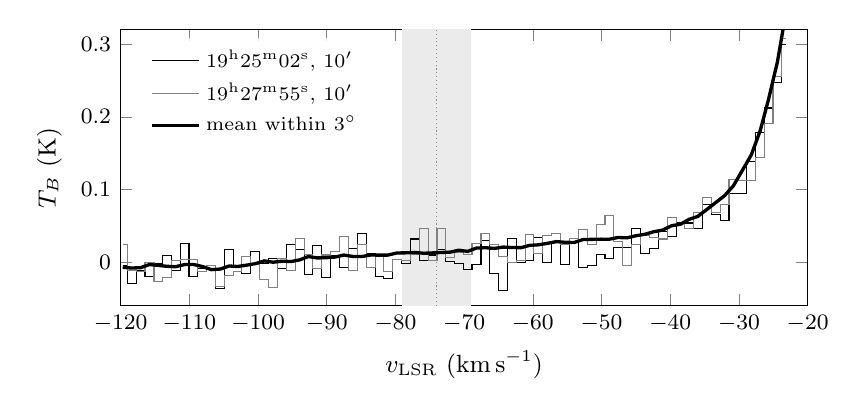
\begin{tikzpicture}
\begin{axis}[width=0.85\textwidth,height=0.42\textwidth,xmin=-120,xmax=-20,ymin=-0.06,ymax=0.32,
  xlabel={$v_\mathrm{LSR}$ (\kms)},ylabel={$T_B$ (K)},tick label style={font=\footnotesize},label style={font=\small},
  legend style={font=\scriptsize,at={(0.03,0.97)},anchor=north west,draw=none,fill=white,fill opacity=0.8,text opacity=1},legend cell align=left]
\fill[black!8] (axis cs:-79,-0.06) rectangle (axis cs:-69,0.32);
\addplot[black!45,densely dotted,forget plot] coordinates {(-74,-0.06) (-74,0.32)};
\addplot[black,thin,const plot mark mid] coordinates {(-119.7,-0.004) (-118.4,-0.029) (-117.1,-0.012) (-115.8,-0.019) (-114.5,-0.002) (-113.3,0.009) (-112.0,-0.011) (-110.7,0.026) (-109.4,-0.019) (-108.1,-0.008) (-106.8,-0.004) (-105.5,-0.036) (-104.2,0.017) (-103.0,-0.005) (-101.7,-0.016) (-100.4,0.015) (-99.1,-0.002) (-97.8,0.005) (-96.5,-0.009) (-95.2,0.024) (-93.9,0.018) (-92.7,-0.017) (-91.4,0.023) (-90.1,-0.021) (-88.8,0.009) (-87.5,-0.007) (-86.2,0.019) (-84.9,0.040) (-83.6,0.012) (-82.3,-0.020) (-81.1,-0.022) (-79.8,0.004) (-78.5,-0.002) (-77.2,0.032) (-75.9,0.003) (-74.6,0.010) (-73.3,0.018) (-72.0,0.001) (-70.8,-0.002) (-69.5,-0.010) (-68.2,-0.003) (-66.9,0.030) (-65.6,-0.016) (-64.3,-0.039) (-63.0,0.033) (-61.7,0.000) (-60.5,0.003) (-59.2,0.034) (-57.9,0.000) (-56.6,0.027) (-55.3,-0.003) (-54.0,0.029) (-52.7,-0.007) (-51.4,-0.004) (-50.1,0.011) (-48.9,0.005) (-47.6,0.020) (-46.3,0.020) (-45.0,0.046) (-43.7,0.012) (-42.4,0.019) (-41.1,0.042) (-39.8,0.036) (-38.5,0.055) (-37.3,0.054) (-36.0,0.046) (-34.7,0.079) (-33.4,0.066) (-32.1,0.058) (-30.8,0.095) (-29.5,0.095) (-28.2,0.138) (-26.9,0.179) (-25.7,0.212) (-24.4,0.247) (-23.1,0.299)};
\addlegendentry{$19^\mathrm{h}25^\mathrm{m}02^\mathrm{s}$, $10'$}
\addplot[black!50,thin,const plot mark mid] coordinates {(-119.7,0.025) (-118.4,-0.011) (-117.1,-0.013) (-115.8,0.000) (-114.5,-0.027) (-113.3,-0.021) (-112.0,0.002) (-110.7,0.004) (-109.4,0.004) (-108.1,-0.013) (-106.8,-0.004) (-105.5,-0.033) (-104.2,-0.018) (-103.0,-0.013) (-101.7,0.008) (-100.4,-0.003) (-99.1,-0.024) (-97.8,-0.035) (-96.5,0.005) (-95.2,-0.011) (-93.9,0.033) (-92.7,0.011) (-91.4,-0.008) (-90.1,0.010) (-88.8,0.015) (-87.5,0.035) (-86.2,-0.011) (-84.9,0.024) (-83.6,-0.007) (-82.3,0.011) (-81.1,-0.013) (-79.8,0.004) (-78.5,0.003) (-77.2,0.011) (-75.9,0.047) (-74.6,0.003) (-73.3,0.046) (-72.0,0.007) (-70.8,0.014) (-69.5,0.011) (-68.2,0.026) (-66.9,0.040) (-65.6,0.024) (-64.3,0.008) (-63.0,-0.000) (-61.7,0.003) (-60.5,0.038) (-59.2,0.012) (-57.9,0.037) (-56.6,0.040) (-55.3,0.025) (-54.0,0.033) (-52.7,0.045) (-51.4,0.024) (-50.1,0.052) (-48.9,0.064) (-47.6,0.028) (-46.3,-0.004) (-45.0,0.024) (-43.7,0.037) (-42.4,0.034) (-41.1,0.032) (-39.8,0.061) (-38.5,0.053) (-37.3,0.046) (-36.0,0.069) (-34.7,0.089) (-33.4,0.069) (-32.1,0.080) (-30.8,0.114) (-29.5,0.113) (-28.2,0.113) (-26.9,0.144) (-25.7,0.191) (-24.4,0.255) (-23.1,0.307)};
\addlegendentry{$19^\mathrm{h}27^\mathrm{m}55^\mathrm{s}$, $10'$}
\addplot[black,very thick] coordinates {(-119.7,-0.0069) (-118.4,-0.0079) (-117.1,-0.0074) (-115.8,-0.0031) (-114.5,-0.0043) (-113.3,-0.0055) (-112.0,-0.0061) (-110.7,-0.0031) (-109.4,-0.0030) (-108.1,-0.0058) (-106.8,-0.0101) (-105.5,-0.0093) (-104.2,-0.0051) (-103.0,-0.0058) (-101.7,-0.0040) (-100.4,-0.0019) (-99.1,0.0019) (-97.8,0.0001) (-96.5,0.0015) (-95.2,0.0010) (-93.9,0.0034) (-92.7,0.0079) (-91.4,0.0060) (-90.1,0.0063) (-88.8,0.0072) (-87.5,0.0100) (-86.2,0.0080) (-84.9,0.0079) (-83.6,0.0100) (-82.3,0.0098) (-81.1,0.0099) (-79.8,0.0128) (-78.5,0.0130) (-77.2,0.0136) (-75.9,0.0124) (-74.6,0.0129) (-73.3,0.0135) (-72.0,0.0140) (-70.8,0.0166) (-69.5,0.0150) (-68.2,0.0196) (-66.9,0.0200) (-65.6,0.0191) (-64.3,0.0209) (-63.0,0.0203) (-61.7,0.0201) (-60.5,0.0232) (-59.2,0.0240) (-57.9,0.0260) (-56.6,0.0284) (-55.3,0.0275) (-54.0,0.0272) (-52.7,0.0313) (-51.4,0.0315) (-50.1,0.0318) (-48.9,0.0317) (-47.6,0.0341) (-46.3,0.0336) (-45.0,0.0365) (-43.7,0.0385) (-42.4,0.0420) (-41.1,0.0443) (-39.8,0.0503) (-38.5,0.0523) (-37.3,0.0589) (-36.0,0.0630) (-34.7,0.0724) (-33.4,0.0820) (-32.1,0.0915) (-30.8,0.1053) (-29.5,0.1264) (-28.2,0.1477) (-26.9,0.1811) (-25.7,0.2237) (-24.4,0.2755) (-23.1,0.3464)};
\addlegendentry{mean within $3^\circ$}
\end{axis}
\end{tikzpicture}
\caption{HI4PI spectra of the two fields averaged within $10'$, and the mean of the
$8826$ pixels within $3^\circ$ of the first, from $-120$ to $-20$\,\kms; the grey band is
$-79$ to $-69$\,\kms\ and the dotted line the signal's $-74$\,\kms. The fields' own
emission, off the plot, peaks at $+3$ to $+4$\,\kms\ with $26$\,K.}
\label{fig:spec}
\end{figure}

% =============================================================================
\section{Related work}\label{sec:related}
% =============================================================================

The Wow!\ signal's sky has been revisited with the Very Large Array~\cite{GrayMarvel2001}
and at the Australian radio telescopes~\cite{GrayEllingsen2002} in search of a
recurrence, and Arecibo Wow!~I and~II~\cite{Mendez2024,Mendez2025} proposed and refined
an astrophysical origin in cold hydrogen. We find no earlier reading of 21\,cm surveys at
the revised fields and velocity.

% =============================================================================
\section{Conclusion}\label{sec:conclusion}
% =============================================================================

HI4PI shows no hydrogen at the Wow!\ signal's revised velocity in either of its candidate
fields: no emission above its noise in the $10'$ averages, no pixel within $3^\circ$ at
five times its own noise, and only the smooth wing of the local emission in the region's
mean. A cloud that fills the $16.2'$ beam at $-74$\,\kms\ is excluded to a column of
$1.4\times10^{17}$\,cm$^{-2}$ in a single channel. A stimulated-emission source that the
Big Ear's beam could catch need not fill HI4PI's, and a compact cloud of angular size
$\theta$ escapes these data below $1.4\times10^{17}(16.2'/\theta)^2$\,cm$^{-2}$, about
$4\times10^{19}$\,cm$^{-2}$ for $\theta=1'$. Interferometric 21\,cm maps of the two
fields at arcminute resolution, which the declination of $-27^\circ$ puts within reach of
the southern arrays, would test the cloud the hypothesis needs.

\section*{Acknowledgements}

This work uses the HI4PI survey through the CDS, Strasbourg, and the software astropy,
astropy-healpix and NumPy.

\begin{thebibliography}{99}\small\raggedright
\setlength{\itemsep}{1pt}

\bibitem{GrayMarvel2001}
R.~H. Gray and K.~B. Marvel, A VLA search for the Ohio State ``Wow'', \emph{Astrophys.
J.} \textbf{546}, 1171 (2001).

\bibitem{GrayEllingsen2002}
R.~H. Gray and S.~Ellingsen, A search for periodic emissions at the Wow locale,
\emph{Astrophys. J.} \textbf{578}, 967 (2002).

\bibitem{Mendez2024}
A.~M\'endez, K.~N. Ortiz Ceballos and J.~I. Zuluaga, Arecibo Wow!\ I: an astrophysical
explanation for the Wow!\ signal, arXiv:2408.08513 (2024).

\bibitem{Mendez2025}
A.~M\'endez, K.~N. Ortiz Ceballos, J.~I. Zuluaga, et al., Arecibo Wow!\ II: revised
properties of the Wow!\ signal from archival Ohio SETI data, arXiv:2508.10657 (2025).

\bibitem{HI4PI2016}
HI4PI Collaboration, N.~Ben~Bekhti, L.~Fl\"oer, R.~Keller, et al., HI4PI: a full-sky
H\,\textsc{i} survey based on EBHIS and GASS, \emph{Astron. Astrophys.} \textbf{594},
A116 (2016).

\bibitem{McClureGriffiths2009}
N.~M. McClure-Griffiths, D.~J. Pisano, M.~R. Calabretta, et al., GASS: the Parkes
Galactic All-Sky Survey. I. Survey description, goals, and initial data release,
\emph{Astrophys. J. Suppl.} \textbf{181}, 398 (2009).

\bibitem{DickeyLockman1990}
J.~M. Dickey and F.~J. Lockman, H\,\textsc{i} in the Galaxy, \emph{Annu. Rev. Astron.
Astrophys.} \textbf{28}, 215 (1990).

\end{thebibliography}

\end{document}
